\chapter[Project Management]{Project Management}
\label{ch:pm}
\containsfigures{Project Management}
%\containslistings{Project Management}
\containstables{Project Management}

\chapterepigraph{Planning is an unnatural process. It is much more satisfying to do something and the nicest thing about not planning is that failure comes as a complete surprise rather than being preceded by a long period of worry and depression.}{Sir John Harvey, c.1800}

\newthought{Project management} is an essential piece of the software engineering process.
Projects must be managed carefully and correctly because of the budgetary and scheduling
constraints they are subject to. Whilst good management does not guarantee the success of
a project, badly managed projects will usually result in failure.

This chapter will discuss the project management techniques used during this project.
It aims to lay out what was planned to help the project be completed successfully, why
these methods where chosen, and how useful they were.

\section{Time Planning}

% Time management techniques used examined, and critiqued

Lorum ipsum sit dolor amet.\citefix{church1932}  \lipsum[2-4]
\section{Development Model}
\label{sec:devmodel}

An agile approach to software development was chosen for this project. This methodology was
chosen because of its focus on rapid development and handling change. When working in a small
team, a heavy weight plan-driven development approach can dominate the actual process of development
due to the overhead. Sommerville states that using such an approach means that ``more time is
spent on how the system should be developed than on program development and testing.''\citepage{sommerville2011}{page 58}
In contrast, an agile approach is designed to deliver working software quickly so that changes
can be suggested and implemented in future iterations.

The agile method that was used was that of extreme programming developed by Kent Beck.\cite{beck1999}\cite{beck2000}
Extreme programming is an `extreme' approach to iterative development. Small releases are made
as quickly as possible. These releases are then evaluated and iterated on until a final release
that meets all requirements is delivered. Instead of planning and designing for the far future,
extreme programming advocates doing both of these activities --- bits and pieces at a time ---
throughout the entire project development lifecycle.

% Bad at frequent, formal release cycle

One core practice at the centre of extreme programming is testing and test driven development.
Test driven development, as described previously in section~\ref{sec:testing}, involves
developing test cases before coding the actual implementation. The benefits of test driven
development are a system that is thoroughly tested, reduced ambiguities in specification before
implementation begins, and avoidance of `test-lag'. However, Sommerville notes a few problems
that can be encountered when using test driven development:

\begin{enumerate}
\item Programmers prefer programming to testing. It is very tempting for a programmer to write
      incomplete tests, or skip test writing altogether, before moving onto the more rewarding
      task of implementation.

\item In some cases tests can be difficult to write. For example, testing user interfaces and
      display logic.

\item It is hard to judge the completeness of a test suite. There may be a large number of tests,
      but do they actually cover all of the code and all possible program execution.
\end{enumerate}

Although the Serenity project does include a test suite the team failed to stick to the test
driven development tenet of extreme programming. This was mainly caused by the first issue
pointed out by Sommerville. The team preferred to go straight into implementing a feature or
enhancement and then, maybe, write tests after the fact.

Another important practice in extreme programming is that of pair programming. Two developers
work in tandem at the same computer. One programmer, the driver, actively writes the implementation
of the program. The other, the observer, continously reviews each line of code as it is typed 
and thinks about the direction of the work.\cite{williams2001} There are a couple of major advantages
to pair programming:

\begin{enumerate}
\item It is an informal code review process that can be very effective at discovering errors
      as the code is written.

\item It promotes collective ownership and responsibility for the component being worked on.
      Code is not `owned' by an individual who may dislike others working in the same area or
      be demotivated by critism during code reviews, similarly one individual is not held responsible
      for any problems.
\end{enumerate}

Studies have shown that pair programming may have little effect on overall productivity, but
creates a substantial reduction in errors in the code.\cite{cockburn2000} This is prescribed
to the continuous code review that occurs, and a decrease in false starts and redoing work.

Pair programming was an effective technique that was used throughout the development of
Serenity. The experience lead to the conclusion that pair programming is a good method for
development for the advantages mentioned above as well as the following reasons:

\begin{description}
\item[Problem solving] When a problem is encountered two people are able to discuss it together
which often helps either or both of them coming up with a solution quicker than they would
individually.

\item[Learning] Knowledge is constantly exchanged within the pair. So after a component
has finished and the pair move on to other work they have both become more effective programmers
in some way.

\item[Team building] Working together lead to better communication and enhanced teamwork.
This made the project team a more effective work group.
\end{description}

However, due to such a small team it was felt that it would be impossible to work on all
tasks in pairs and still finish the work within the time constraints. Therefore, some work
was done individually, but still always trying to work in close proximity to enable teamwork
where necessary.

\section{Project Control}
\label{sec:control}

% Control Measures examined and critiqued
% ie change requests

Projects that have run late or overbudget often find that the steps to failure happened gradually.
The small extra costs or wasted days gradually added up to form a very large and significant
problem. Project control is about detecting these small deviations and then implementing corrective
actions that prevents a build up of small problems.\citepage{maylor2010}{page 291}

Any large software system is going to undergo change as it is developed. Requirements may change,
bugs have to be fixed as they appear, and original design decisions may turn out to be insufficient.
Therefore, a set of change management processes are required to ensure that the evolution of a
system is controlled and does not succumb to scope creep or other problems that would prevent
successful delivery of the software.\citepage{sommerville2011}{page 685}

For the Serenity project the change management process shown in Figure~\ref{fig:change_management}
was devised. This protocol was designed to allow stakeholders outside of the development team
to submit change requests for assessment. When a change request is received it would be evaluated
in terms of its cost and impact on the project requirements. If the change is accepted then a
notification is relayed to the whole development team and relevant stakeholders. All change requests
would be archived so that reasons for rejection or approval could be reviewed again in the future.

\begin{figure*}
	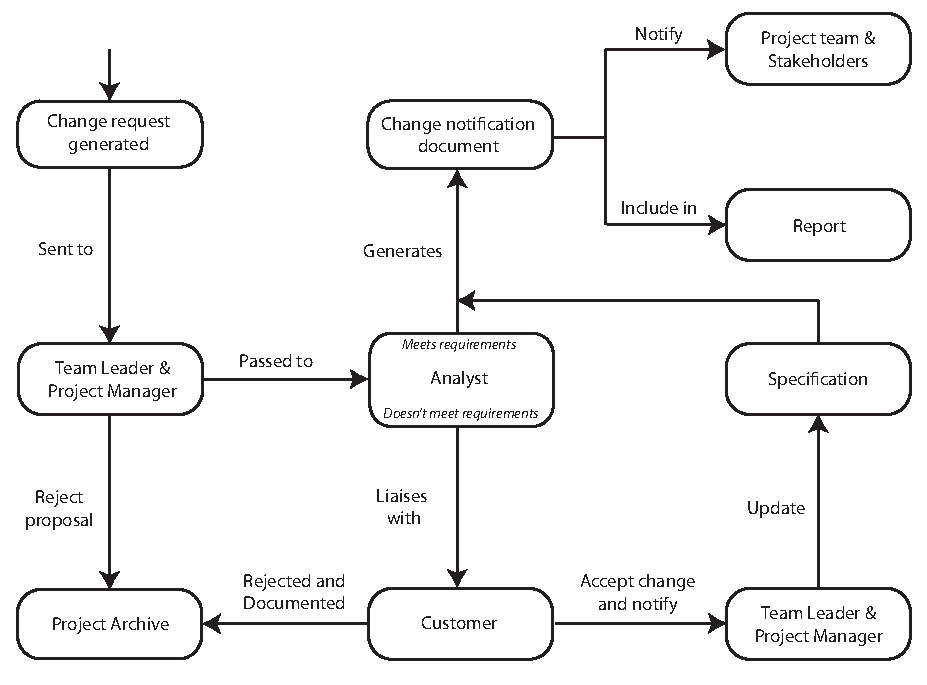
\includegraphics[height=33em]{res/change_management_diagram}
	\label{fig:change_management}
	\caption{Change management workflow}
\end{figure*}

In the end no change requests were submitted by any stakeholder not a part of the development team.
However, it is believed that this well documented and rigorous change management workflow would
have enabled the project to deal with any such change requests in an efficient manner.
Many minor changes, such as bug fixes, were discussed more informally within the development as
they had no effect on the schedule or requirements. This worked effectively whereas using the
formal change management procedure for such small changes would be overkill and lead to a lot
of time being wasted in communications overhead.

% Major changes? E.g. scaling back the goals to get a finished product.

A formalised change management workflow is necessary for a successful project, but it must only
be used where appropriate to ensure that it does not get in the way of smaller changes that
can be dealt with more informally.

\section{Stakeholders and Communication Plan}
\label{section:communication}

The various parties identified as stakeholders are shown in table \ref{tab:stakeholders} below. The relationship between the stakeholder and the project is shown, along with a rough estimate of their power and interest.\sidenote[][-2em]{See \bibentry{mendelow1991stakeholder}} This grid will form a reference for making sure that all interested parties are communicated with appropriately throughout the duration of the project.

\vspace{1em}

\begin{table*}
	\small
	\renewcommand{\arraystretch}{1.6}
	\begin{tabular}{p{9em} p{5em} p{2.5em} p{2.5em} p{9em} p{9em} p{8em}}
		\toprule
		\emph{Stakeholder} & \emph{Relationship} & \emph{Power} & \emph{Interest} & \emph{Requirements} & \emph{Measurements} & \emph{Communication Strategy} \\
		\midrule
		
		Project Team & Internal & High & High & 
		Good working environment, creative input. & 
		Meeting project spec, good grades! & 
		Various, detailed elsewhere. \\
		
		Supervisor --- Sara Kalvala & Internal & High & High & 
		requirement & 
		Adherence to spec, good PM, high quality write-up. & 
		Weekly meetings. \\
		
		Client --- Matt Leeke & Core \mbox{External} & High & High & 
		requirement & 
		measurement & 
		Weekly meetings. \\
		
		Second Assessor & Core \mbox{External} & High & Low & 
		requirement & 
		measurement & 
		Deliverables only. \\
		
		Projects Organiser --- Steve Matthews & External & High & Low & 
		requirement & 
		measurement & 
		Email or meeting if required. \\
		
		Playtesters & External & Low & High & 
		requirement & 
		measurement & 
		Email. \\
		
		Other future users & Rest of World & Low & High & 
		requirement & 
		measurement & 
		Website, forums, blog. \\
		
		The Haskell and FP Communities & Rest of World & Low & High & 
		requirement & 
		measurement & 
		Online as above, and via the final report. \\
		\bottomrule
	\end{tabular}
	\vspace{1.5em}
	\caption{Stakeholders for the project.}
	\label{tab:stakeholders}
\end{table*}

\noindent Communication within the project team is examined in detail elsewhere in this document, so the remainder of this section is concerned with the other stakeholders.

\subsection{Supervisor Meetings}

Regular communication with the project supervisor is likely to be a critical factor in success of the project. For this reason a weekly meeting with at least one member of the group if not more will be high priority.

\subsection{Client Meetings}

The client is clearly vital to the success of the project, and continual feedback on each release will allow for early identification of any problems. At least one meeting per release (ie each week) will be required, as well as further meetings and correspondence as needed.

\subsection{Projects Organiser and Second Assessor}

The projects organiser could exert a strong influence over the project if they wished, but as there are many projects and it would be inappropriate for them to demonstrate partiality, extended levels of communication are unlikely to be necessary. Brief updates pertaining to deliverables is all that should be required. But if the project organiser initiates communication then they should be made a high priority.

Communication with the second accessor is, for the most part, not appropriate, excepting when within the remit of the deliverables, i.e. the report and presentation themselves.

\subsection{Playtesters and End Users}

\subsection{The Haskell and Functional Programming Communities}

The overall end goal of the project is not just a game, but an examination of Haskell and Functional Programming as a game development environment. 



\section{Team Structure}

Before starting the development phase of the project the roles and responsibilities for
each team member were formalised. Each person was given a set of roles and responsiblities
for which they would be primarily in charge of. It was envisaged that these roles would
be flexible and that responsibilities would be shared, but having a formal specification
of the member ultimately responsible for an aspect of the project's development and management
would be useful for ensuring that everything was done correctly. The roles that were given
to each team member as laid out in the specification are as follows.

\subsection{Laith Alissa}
\begin{description}
    \item[Project Manager] Responsible for overseeing the human aspects of the project in general, including managing a schedule, organising meetings and collaborative development sessions. Makes decisions involving tradeoffs between project time, cost, and quality.
    \item[Customer Liaison] Meets with the customer at regular intervals to discuss the project progress, outlook, and any issues which are require customer input. 
    \item[Analyst] Responsible for ensuring the customer requirements are addressed during planning and development stages of the project, and ensures that the solution will sufficiently address the customers needs.
    \item[User Manager] Responsible for communicating with play-testers and users. Finds end users to test the product in the later stages of development, and provides feedback to the project team. Prime responsibility is to identify issues which are not clearly visible from the project development perspective, but are more apparent to end users. 
    \item[Graphic Designer] Responsible for prototyping and developing graphical design elements, such as ship sprites, terrain, maps and user interface.   
\end{description}

\subsection{Jon Cave}
\begin{description}
    \item[Code Reviewer] Responsible for interpreting other developer's code, checking for logical inconsistencies and familiarising themselves with the project as a whole.
    \item[Chairman] Responsible for coordinating meetings, ensuring all issues are resolved or at the least discussed, and that all meeting participants have a chance to voice concerns and contributions.
    \item[Testing and Integration Officer] Ensures the code is thoroughly tested for bugs, and discovered bugs are flagged and dealt with in reasonable time. Responsible for managing integration testing to prevent bugs occurring on the master branch.
    \item[Security Officer] Checks for security flaws in the product, performs security evaluations (such as penetration testing and code review) to ensure the product is sufficiently secure.
\end{description}

\subsection{Joseph Siddall}
\begin{description}
    \item[Software Librarian] Ensures team completes documentation to a sufficient standard for long term maintenance. 
    \item[Line Manager] Oversees day to day development, intervenes if a developer is off track, ensuring minimal time is wasted perusing low priority work.
    \item[Testing and Integration Officer] Ensures the code is thoroughly tested for bugs, and discovered bugs are flagged and dealt with in reasonable time. Responsible for managing integration testing to prevent bugs occurring on the master branch.
\end{description}

\subsection{Victor Smith}
\begin{description}
    \item[Team Leader] Leads the project. Responsible for coordinating the project team, ensuring team members are working to the best of their ability, responsible for making decisions when the there is no clear solution to a particular problem.
    \item[Lead Developer] Responsible overall for technical areas of the project. Consults other developers when there is development difficulty, also responsible for directing programming style and technique.
    \item[Composer] Composes soundtrack for the game, and produces required sound effects, voice overs, soundscapes, and other related resources.
\end{description}

\subsection{Common Roles}

Some of the roles were shared by the whole project team. This is because all of the
team members were involved in day to day development and game play design.

\begin{description}
    \item[Programmer] Performs the day-to-day programming specified by the line manager.
    \item[Tester] Performs general code testing (e.g.\ unit tests, component tests).
    \item[Gameplay Designer] Critically analyse gameplay design and experience, giving feedback to the team leader on how to improve the game's appeal.
\end{description}

\section{Risk Management}
\label{section:risk}
 
A proactive approach to risk management was taken. This technique was chosen in order
to maximise the probability of avoiding risks instead of having to move into `fire-fighting mode'
if something went wrong.\citepage{pressman2010}{page 745}
 
As part of this proactive risk management strategy, a number of potential risks were identified.
These risks are shown in table~\ref{tab:risks} along with their estimated probabilities of occurring
and impact if they were to occur.
 
\begin{table*}
	\small
	\begin{tabular}{l p{\textwidth / 2} l l}
		\toprule
		\emph{Risk} & \emph{Description} & \emph{Probability} & \emph{Impact} \\
		\midrule
		Length underestimate & The time required to develop the software is underestimated & Medium & High \\
		Team member illness & One or more team members unable to work due to illness & Medium & High \\
		Hardware failure & Damage to critical hardware causing loss of data & Medium & Medium \\
		Size underestimate & The size of the deliverable has been underestimated & Medium & Medium \\
		Requirements change & Large number of changes to requirements during development & Low & Medium \\
		Ambiguous requirements & Requirements are not fully understood or misinterpreted leading to
			loss of development time as the specification is recreated & Low & Medium \\
		\bottomrule
	\end{tabular}
	\vspace{1.5em}
	\caption{Risk identification and analysis.}
	\label{tab:risks}
\end{table*}
 
With the risks identified, and their likelihood and consequences estimated it is necessary
to draw up plans to mitigate their effects. There are three types of management strategies 
for individual risks: avoidance strategies to reduce the probability of the risk occurring;
minimisation strategies to reduce the impact of the risk; and contingency plans to deal with
the risk if it does arise.\citepage{sommerville2011}{page 601} It is best to avoid the risk,
but if this is not possible then minimisation of the effects and, finally, contingency plans
should reduce the overall impact of a risk on the project. The mitigation and management
strategies for each risk previously identified are listed in table~\ref{tab:rmm}.
 
\begin{table*}
	\small
	\begin{tabular}{l p{37em}}
		\toprule
		\emph{Risk} & \emph{Mitigation / Management} \\
		\midrule
		Length underestimate & Detailed work breakdown with weekly releases to ensure that
			schedule slippage can be caught early \\
		Team member illness & Well documented code (enforced by the software librarian) so
			that other members can quickly start work on less familiar sections of
			the codebase \\
		Hardware failure & Backups and distributed source control, see section~\ref{section:tools} \\
		Size underestimate & Detailed work breakdown structure \\
		Requirements change & Thorough change management system, see section~\ref{section:control} \\
		Ambiguous requirements & Thorough planning phase \\
		\bottomrule
	\end{tabular}
	\vspace{1.5em}
	\caption{Risk mitigation and management.}
	\label{tab:rmm}
\end{table*}
 
The final stage of the risk management process is monitoring. Throughout the duration of
the project each identified risk was reassessed for changes to its probability and
impact. This allowed the mitigation and management strategies to be revisited to ensure that
they were as effective as possible.
 
The two previously identified risks that actually occurred were team member illness and length underestimate.
On a couple of occasions a team member was ill and unable to attend group work sessions or work to their full
capacity. Fortunately, the team was able to reduce the impact of this by ensuring that the work each individual
was performing was not hindered by an absence. This was done by allocating work tasks to be as separate as
possible to allow more parallel development to occur. Also, an illness was never so severe as to stop a team
member from working for longer than a day or two. However, the issue of length underestimation was more serious.
 
% Length underestimation
%
% 1. More time required for network and GUI than hoped
% 2. (1) slowed the development of the ideal game
% 3. (1) was very informative for our goal of investigation of Haskell for game development
 
The proactive approach to risk management was a good choice. By reviewing the potential
risks before starting the development phase of the project it was much easier to avoid risks that could
have had disastrous consequences for the project. For example, by implementing a thorough backup strategy
prior to any data loss actually taking place it was ensured that no work would have been lost if a hardware
failure had occurred. Continuously monitoring and reassessing these risks was also helpful in preventing
any risks becoming more probable or having a greater impact.

\section{Legal, Ethical, and Social Issues}
\label{sec:legal}

Prior to embarking on this project several potential professional issues were identified
and discussed to ensure that they were addressed appropriately.

Any software project faces issues surrounding copyright and intellectual property. During
development the team were aware that all third party libraries used in the project must
be licensed appropriately. This meant only using software with a permissive license (e.g.
Apache, BSD, or MIT licenses) and no unlicensed proprietary software. It was also important
to avoid infringing on the intellectual property of established game publishers and their
existing games. Obviously it was infeasible to review all previously published games to
check if Serenity bears great similarities to any of them. However, the project team was
careful not to directly copy any designs or unique game play characteristics of existing
games that they are familiar with.

The games industry is faced with several ethical and social issues that were thought about
carefully when designing the Serenity game. Highly controversial issues that surrounds
current games, such as racism and violence, were thought about carefully and it was ensured
that they would not be issues with the Serenity game. This is because the game is based
in a fictional world with a very unrealistic graphical representation. Another social
dilemma for game creators to consider is that of the addictiveness of their creations.
Players often invest many hours, often consecutively, in playing games and can even spend
large sums of money on pay-to-play games. The game that was developed was designed to
have short playing periods that would allow convenient times for the player to quit.

\section{Evaluation of Tools and Techniques}
\label{sec:tools}

A number of different tools were used in the day to day running of the project.
These tools were used to ease the collaboration between members by ensuring that everyone knew
what they were supposed to be doing and how to share it with the others.

\subsection{Source Control: Git}

Source control systems are an essential tool for software projects, especially those
with multiple developers. Using source control to easily track the changes to source
code is helpful because, as McConnell explains, having a history of changes helps a
developer to identify the origin of bugs quickly.\citepage{mcconnell2004}{page 667}

The Git source control system\sidenote{\url{http://git-scm.com/}} was chosen for this project.
Git was chosen for a number of reasons. Firstly, it has a lightweight branching model which
allows for quick creation of new development branches for experimental features independent of
any other development. Chacon notes this as Git's ``killer feature''.\citepage{chacon2009}{page 38}
Another reason for choosing Git is its distributed nature. Every user has a full clone of the
entire repository that can act as a replacement for any other instance of the repository; this means
that there is no single, centralised point of failure.

A centralised master repository was hosted on Github, a popular code host.\sidenote{\url{https://github.com/}}
This made it easier for team members to share their changes to the code base. Once a change has been made
it can be `pushed' to the Github repository; other team members can then `pull' it to their local
repositories.

Git was an ideal source control system for the project. Not only does it allow the users to see
the entire history of changes made to the project it makes collaborative development between
multiple team members incredibly easy. Instead of having to resolve conflicting changes to files
it is possible to use the built in merge tool to combine the work of two or more people on the
same set of files with minimal effort. Git is recommended for all future development projects.

\subsection{Tracking and Managing Releases: Trello}

\begin{marginfigure}
	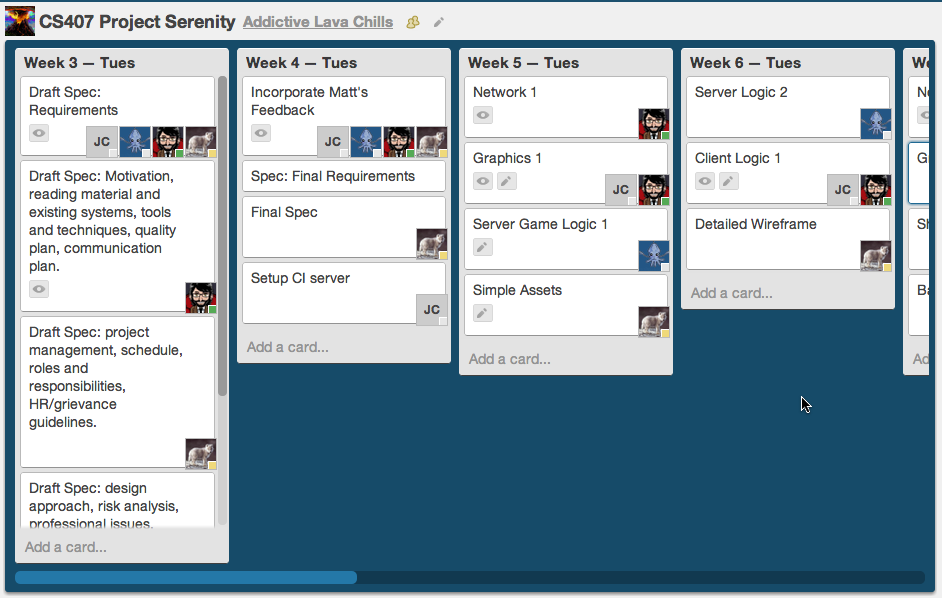
\includegraphics[width=6cm]{res/trello.png}
	\caption[Trello]{Project Serenity's Trello page}
	\label{fig:trello}
\end{marginfigure}

Trello is a modern, online take of an age old concept --- a wall of post-its. Trello allows for overall planning of tasks and communication between members in a highly dynamic, fluid way. Cards are arranged into a list-of lists, each list being some kind of functional decomposition or `stovepipe'. Trello has been used in the project to track the requirements for each weeks releases, but still allowing rapid changes to be made and communicated.

Trello acted as a useful reference to the current state of the project: what tasks are planned and who is doing them.
It is a good tool for keeping a small group of people organised, but requires careful management to keep it
up to date and useful.

\subsection{Bug Tracking: Github Issues}

Trello does not entirely alleviate the need for a full bug tracker. When working of development of
individual features and components it was necessary to have a method of tracking more transient issues
and tasks. The initial plan was to use the service provided by Fogbugz, a stand alone bug tracking
web application. However, in the end the Issues feature built into Github hosted repositories was
used. This was decided because it reduced the number of third party services that were relied upon
and it provided better integration with the hosted repository itself. Although it is much more minimal
than Fogbuz, it provided enough features, such as milestones, labels, email notifications, and
issue assignment, for this project.

An issue tracker was very useful for noting down smaller tasks and bugs that cannot be fixed immediately,
but must not be accidentally forgotten about. If a project is using Github to host code then the
Issues component is recommended if only simple issue tracking features are required. However, for
more complex requirements a more fully featured service may be a better option.

\subsection{Backups}

Backups of the source code and other project assets are essential. In the event of a
disaster, such as losing a computer to a fire, it must be possible to recreate the
entire project in its latest state quickly and without any repetition of work.\citepage{mcconnell2004}{page 669}
The use of Git and Github for source control made it simple to ensure that all
source code was located on multiple computers. By `pushing' commits to the Github
repository all code was stored in the cloud. When other team members `pulled' the code
later on it was then mirrored on their computers as well. Extra precautions were taken
by also `pushing' the Git repository to private servers owned by the team members.
Also, the free service provided by Dropbox\sidenote{\url{https://www.dropbox.com/}}
was used to share and backup any other files, such as assets and planning notes.

Fortunately a situation which required recovery from backups was never encountered,
but the strategies put it place should have been more than adequate if the need ever
arises in the future. Since the main backup strategy was part of normal development
workflow it was impossible to forget to implement it. However, it does have to be ensured that
all members are sharing their changes as frequently as possible (even if a feature is
not fully finished) to prevent any work in progress from being lost in case an individual's
computer dies. The extension to this core backup strategy, storing the repositories
on other personal servers, was easy because of Git's feature set which was designed
to be distributed in nature and so allows tracking and updating of multiple remote repositories.

\subsection{Continuous Integration: Jenkins}

Section~\ref{sec:testing} introduced the idea of continuous integration as a method
of regularly running the test suite and performing a full build of the software.
The Jenkins continuous integration server\sidenote{\url{http://jenkins-ci.org/}}
was used for this project. Jenkins was chosen because it is a widely used open
source project.\sidenote{\url{http://stats.jenkins-ci.org/jenkins-stats/}}
Jenkins also works well with projects hosted on Github because of its Github plugin\sidenote{\url{https://wiki.jenkins-ci.org/display/JENKINS/GitHub+Plugin}}
and Github's Jenkins specific post-receive hook.

Although Jenkins does not have a very good user interface it suited the needs of
this project. It was a good tool for running a test suite with every change to the
code base and ensuring that the game would build correctly. Email notifications on failure
were useful, but also relatively noisy at times. Continuous integration is probably
more useful for more mature projects that need to ensure that changes do not introduce
any regressions than it is for a project in the early stages of development when a lot
of features are not fully working.

\chapter[Requirements]{Functional and Non-Functional Requirements}
\label{ch:requirements}

\chapterepigraph{``All things are created twice; first mentally; then physically.  The key to creativity is to begin with the end in mind, with a vision and a blue print of the desired result."}{ Stephen Covey}

\newthought{Starting a sentence} with a new thought.


% help site at http://www.projectmanagementhelp.com/how-to-write-functional-requirements/
% bullet point these requirements, describe them, specify any details.
% include bain quite as footnote
\section{Functional Requirements}




\section{Non-Functional Requirements}


functional - 2d, realtime strategy, multiplayer, ship design, resource system, ai, planetary capture resource system, possiblity of campaign style multiplayer, tactical zoom/gameplay, fow, hw requirements, haskell.
non-functional - fun, reliable, secure, short lived game sessions, 

\section{Evaluating the Success of the Project}

Project success depends highly upon perspective, one stakeholder might consider the project beyond successful whereas another stakeholder may consider the project a total failure. Evaluating success must consider a variety of perspectives, and even then it may not be as simple as a yes or no answer. 

\begin{quote}
An architect may consider success in terms of aesthetic appearance, an engineer in terms of technical competence, an accountant in terms of dollars spent under budget, a human resources manager in terms of employee satisfaction, and chief executive officers rate their success in the stock market.
%todo reference Freeman and Beale (1992,p. 8) 
\end{quote}

%todo: this is vics stuff, didn't even proof it, shot-not (Laith),
\paragraph{Shenhar et al, 1997} \cite{shenhar} In this paper it is suggested that the traditional measures of project success --- namely time cost and quality --- are perhaps not the best, and points out the disagreement in the literature on this area. Building on evidence from previous studies, the authors suggest a new, multidimensional, framework for project success; and, notably, back this up and expand upon it by utilising empirical evidence.

This evidence takes the form of 127 structured questionnaires, returned from project managers from a variety of industries.\sidenote[][-6em]{It is claimed in the paper that despite this selection having not been made at random, with no consideration to stratification, and that 'the end products were aimed at a military market', that there is not an inherent bias. Especially in light of the low sample size this should be considered to be a somewhat dubious claim.} This data was then analysed using numerical measures from previous work\sidenote[][1em]{Specifically Cooper and Kleinschmidt, 1987;  Pinto and Stevin, 1988; Stuckenbruck, 1986; and Dvir and Shenhar 1992. (See full bibliography).} and the dimensionality of results determined using factor analysis.\sidenote[][1em]{Factor analysis being a statistical technique to determine the underlying dimensionality of a data set without previous knowledge of it. See Brayant and Yarnold (detail in bibliography) for a full treatment.}

Despite an initial hypothesis of three dimensions to project success, the analysis suggests that there are in fact four. These dimensions were then correlated(using Pearson's Correlation) with the overall assessment of project success, with favourable results; and the relative strength of each measured, both for projects in progress and completed projects. The strength was seen to be consistent, apart from the fourth dimension which was significantly better correlated in completed projects. This is the 'future potential' dimension. 

This empirical experiment causes this research to stand out in a way other papers on the subject of project success do not, in that the claims are in fact backed up. This is in sharp contrast to Atkinson's paper (see below).

Another notable feature of this paper is that in addition to the scientific numerical approach, a significant percentage of the text is given to practical consequences of the results and implications for the practitioner. Given that it is now nearly fifteen years old it is surprising that these ideas do not feature more prominently in project management canon.
%
%In the paper ``Project management: cost, time and quality, two best guesses and a phenomenon, its time to accept other success criteria'' %todo citation
%, Atkinson considers typical assessment criteria to be insufficient, and proposes a new method known as "The Iron Triangle" which aggregates many existing paradigms to form a new way of evaluating project success.
%
%In the paper ``Mapping the dimensions of project success'' Shenhar et. al. identify four dimensions which measure the success of a project, and can be further used to quantify the success of a project against a benchmark of well known projects throughout history.
%


The Iron Triangle is a primitive tool for measuring the balance between time, cost and quality. It has no quantifiable properties and is mainly an illustrative tool, but it does somewhat accurately express the relation between the three constraints.
\begin{marginfigure}
	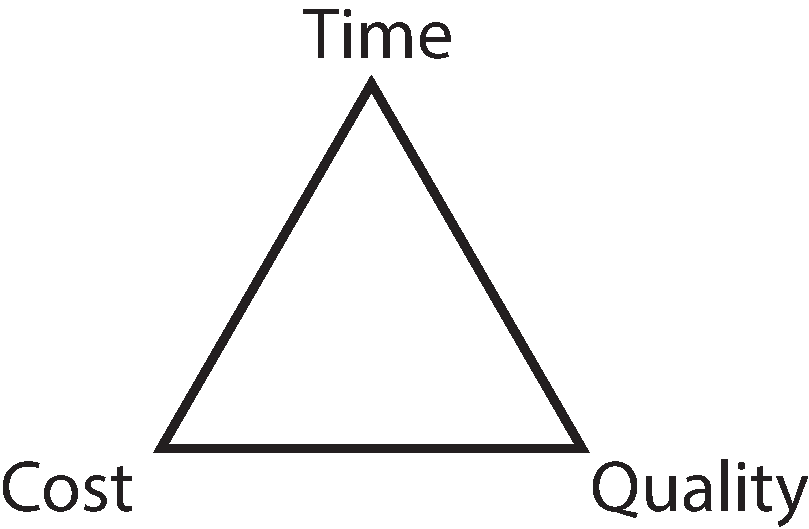
\includegraphics[width=55mm]{res/pm/TCQ_triangle}
	\label{fig:TCQ_triangle}
	\caption{The Iron Triangle}
\end{marginfigure}
Selecting two of the properties as desirable will be costly to the third, for example demanding a high quality product in little time will escalate the cost. The project had no real notion of monetary cost, so the balance was largely between quality, project time and personal time, where the personal cost a team members marks from other assignments, time for hobbies, sleep, etc. For almost all project components there would be an imbalance between the three properties, and most often, the \emph{personal time} property would need to be increased to ensure good quality products while keeping to schedule.  


\paragraph{Success Dimension 1 : Project Efficiency}
The first dimension is interesting in the way it applies to software projects, since efficiency is extremely difficult to guage. Unlike a task requiring manual labour, efficiency can be assessed fairly easily since most tasks are repeatable and hence can be modelled fairly easily. It's difficult, on the other hand, to compare two software projects, since not only are they very rarely alike, but efficiency is not easily quantifiable. Some managers try to quantify development progress by measuring lines of code per day, as Hertzfeld implied in his article ``-2000 lines of code'', the number of lines a developer has written per day may have no bearing on the work accomplished. Even it there was a convenient function of project progress to mark efficiency, that efficiency would likely be subject to changes. Suppose a large software project launches, stays on schedule and outputs an excellent number of lines per day, it might be the case that the developers are taking shortcuts and not being prudent, which could cause a massive slump in the efficiency late down the line when it's discovered that the initial few milestones are bug ridden and need to be revised. By contrast a project team missing the initial deadlines might be investing a large amount of thought into their work which could accelerate their efficiency later down the line. The important thing to note is that efficiency hinges on perspective, and it's very difficult to find a function to assess the efficiency of a software project.
%%todo: Sounds sloppy so far, revise!
Given that it is in fact necessary for the model, it would be wisest to measure efficiency by comparing each estimated milestone completion date with it's actual completion date, since the milestones were all met on time, but some features were lacking, it's fair to claim the project progress was reasonably efficient \emph{efficiency} available. 

\paragraph{Success Dimension 2 : Impact on customer}
%todo: Matt's feedback?

\paragraph{Success Dimension 3 : Business and Direct Success}
Business and Direct success is a measure of whether the project provided ``the sales, income, and profits as expected'', ``increase[d] business results'' or whether the project ``helped to increase market share'' \cite{shenhar}. Shenhar does elaborate that other projects may not fall under the same assessment criteria, but will have some mechanism of measuring direct success. Since this project is academically motivated rather than monetarily driven, it would be fair to assess the success outcomes the requirements discussed in section \ref{sec:reviewrequirements}. The project met most of these requirements, and the requirements it failed to meet were considered the least important. The project was largely successful in creating a fun game in Haskell, which met almost all the functional requirements and fulfilled all the non-functional requirements, granting the project at least a partial success under Dimension 3.
 
\paragraph{Success Dimension 4 : Preparing for the Future}
The fourth dimension investigates how prudent the project is, whether it has invested in future opportunities, whether it explored further ideas, innovations or skills which may be required in the future. Assessment under this dimension can only result in an overwhelming success. The project explored two concepts which are already hugely popular and only growing in popularity, namely indie games and the Haskell programming language. Haskell's growing popularity is undeniable, it's a concise yet extremely powerful language which has recently being adopted by an increasing number of companies including ABN AMRO, Anygma, Amgen, Bluespec and Eaton. It has been used to construct many large scale projects such as ASIC, FPGA (design software), Haskore, GHC, Darcs and HAppS, projects which are of comparable size and complexity of many corporately produced games. \cite{realworldhaskell}

%todo: Probably won't be able to phrase of cite this bit properly tonight
Game development is also a very rapidly growing market, with the advent of mobile devices the target audience for video games barely excludes any social group.  
% Can't think of how to finish this
The project has produced a wealth of experience for developing games in Haskell...

\paragraph{Overall Success}
Each dimension is a measure of success for a time frame, the first being concerned with the immediate results of the project, the fourth being concerned with the distant future and the interactions the project may be a part of in the future. This project was by no means perfect, but it showed strong signs of success when applying Shenhar's success measurement criteria.


\section{Conclusions}

\begin{itemize}
\item Assessment of our key decisions
\item Conclusions on Haskell
\end{itemize}

